% time values for run2 and run3
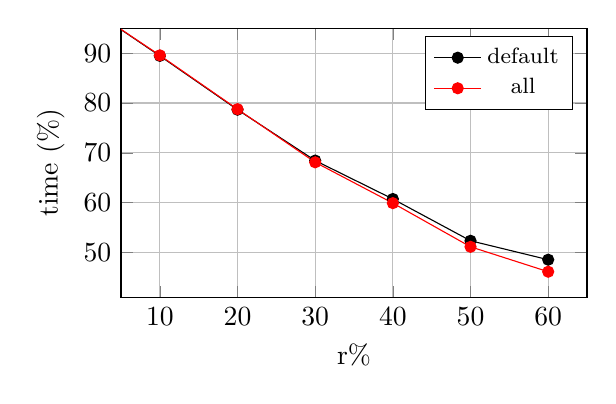
\begin{tikzpicture}
\begin{axis}[
    title={},
    height=5cm,
    width=7.5cm,
    xlabel={r\%},
    ylabel={time (\%)},
    xmin=5, xmax=65,
    ymin=41, ymax=95,
    xtick={10,20,30,40,50,60},
    ytick={50,60,70,80,90},
    legend pos=north east,
    xmajorgrids=true,
    ymajorgrids=true,
    legend style={font=\footnotesize}
]

\addplot[
    color=black,
    mark=*
    ]
    coordinates {
    (0,100)(10,89.45)(20,78.65)(30,68.45)(40,60.74)(50,52.36)(60,48.56)
    };
    
\addplot[
    color=red,
    mark=*
    ]
    coordinates {
    (0,100)(10,89.56)(20,78.76)(30,68.10)(40,59.91)(50,51.15)(60,46.15)
    };
    
\legend{default, all}
    
\end{axis}
\end{tikzpicture}